\chapter{Object Detection, Tracking and Labelling}

The main task of this dissertation is focused on the detection, tracking and labeling of objects in motion found in the field of view of the several sensors equipped in ATLASCAR 2. In this chapter it will be succinctly explained how these features were implemented. 

Firstly, it will be described how the detection and tracking in the image is performed. In the image tracking phase happens also the labelling phase and the creation of dataset files and image templates. 

Secondly, the implementation of the tracking of multiple targets with ranged based sensors will be explained. To make this step possible, the \gls{mtt} library designed by Almeida \cite{SoaresDeAlmeida2016a} was used. The \gls{mtt} library contains methods of perception and planar object detection. 

Lastly, the multi-modal approach will be used where both data from the images and the \gls{lidar}s will be assembled and a single perception unit will be created. With this conceptualization, it is possible to detect, track and label objects easily in the ATLASCAR 2.

The image sequences and laser scan data obtained for the development of this stage of the dissertation were recorded into rosbags using the ATLASCAR 2 using the sensors it has. The rosbags were recorded in October 17, 2017, in the afternoon. Two rosbags were recorded:

\begin{itemize}
	\item The first rosbag was recorded while leaving Departamento de Engenharia Mec\^anica at Universidade de Aveiro. The car travelled around the campus and visited the Alboi neighbourhood.
	\subitem In this bag there are cars, vans, cyclist and pedestrians. It is a bag where the car also runs into slopes. It is a rosbag with more detail which was used later in the project.
	\item The second rosbag starts at Alboi where the first rosbag stopped. The car follows a path into the A25 highway until the first exit.
	\subitem There are mostly cars in this one and it was a good rosbag to start with some tests in tracking objects.
\end{itemize} 

\section{Image Tracking}

The development of object detection, tracking and labelling starts by processing and analyzing the image sequences. A labelling node was created in \gls{ros} where the features in this chapter were implemented. This node subscribes to the camera images through its rostopic. In resemblance to the calibration, the image comes encapsulated in a \gls{ros} message to be processed in a callback function. In this function the image is analyzed.

\subsection{Template Matching}

The image is converted from the \gls{ros} message format into an \gls{opencv} format so it can be easily manipulated. \gls{opencv} treats images as matrices of pixel with $(x,y)$ coordinates and RGB values. As the image sequences arrive, they are stored into a queue. This queue will be used later to look back to the previous frames and back-track the object. 

When the node starts, a window opens (see figure \ref{fig:view}) for the user to view the video stream recorded in the bag. The node also functions in real-time. In other words, the node can be executed by connecting the computer directly to the car, obtaining the images in immediately. In this window, the user can click on objects that may appear. To obey the scope of the dissertation, most of the objects captured were cars, vans and people. Some street signs were also tested. When the user clicks on an object, a callback function is triggered to process the mouse event and a bounding box appears around the selected target.

\begin{figure}[htp]
	
	\centering
	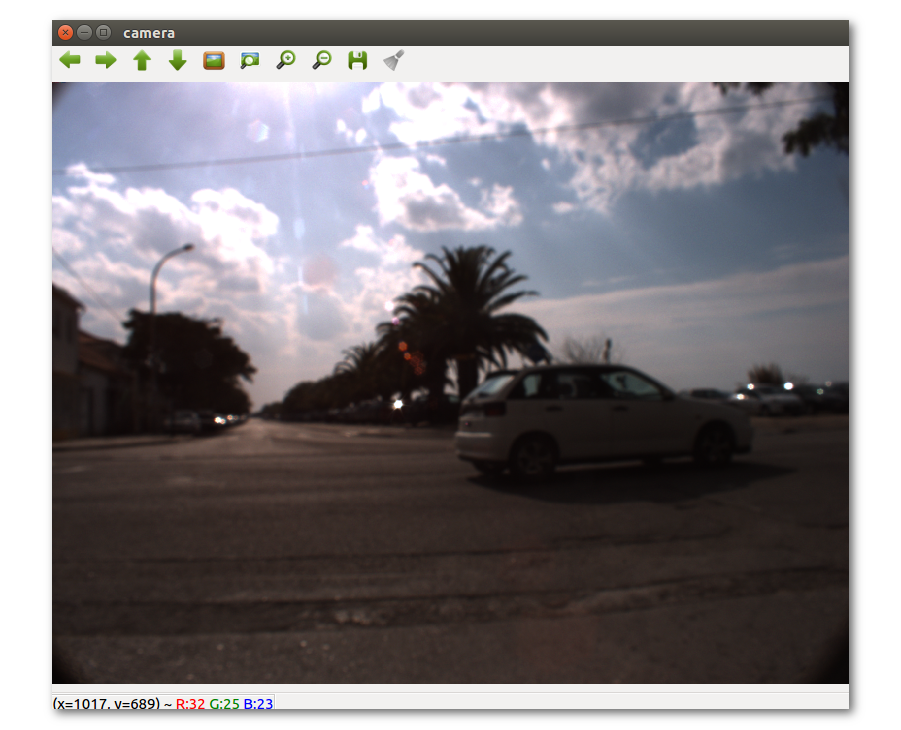
\includegraphics[width=0.8\textwidth]{caplabel/imgs/view.png}
	
	\caption{Window view with image sequences appearing}
	\label{fig:view}
	
\end{figure}

This callback function gets the $(x,y)$ coordinates of the mouse click. The bounding box size is given by the distance to the object. If the distance is greater, the bounding box will be smaller and vice-versa. The distance to the object is given by the tri-dimensional spacial coordinates given by the \gls{mtt} library explained further in the dissertation. This library uses the \gls{lidar} sensors of the ATLASCAR 2, and since it was developed specifically for the ATLASCAR it is the optimal tool to detect and track objects in the field of view.

The upper third-part of the image is ignore as it is considered to be irrelevant content as most of it will be tall objects like trees or objects in the sky, like clouds. Also, it is meant for the image to be fused with the laser data, and since the ATLASCAR 2 is equipped with planar based sensor, the objects off the ground will be out of the scope. The bounding box tracks the object inside the bounding box. To accomplish this, template matching techniques are used. Firstly, the previous frames are saved. The node will check the queue of previous frames and store them to use them later. 

The template matching strategy is used to track the selected target in the next frames. It begins by copying the source image to display to another \gls{opencv} matrix and also creates a result matrix. The matching is now performed using a method implemented by \gls{opencv} called \texttt{matchTemplate} which takes the source image, the patch (which is the \gls{roi} inside the bounding box), the result matrix and a matching method. 

Template matching is a technique for finding areas of an image that match (are similar) to a template image (patch). It is needed a source image which will be the actual frame and a template image which will be the \gls{roi} in the bounding box. The template matching purpose is to detect the highest matching area. to identify the matching area, the algorithm compares the template image with the source by iterating it through the source image. In other words, the patch will move on pixel at a time in the source image  (left to right, up to down). At each cycle, a score is calculated. This score represents how good the match is in that position of the source image (or how similar the patch is to that particular area in that location). 

\begin{figure}[htp]
	
	\centering
	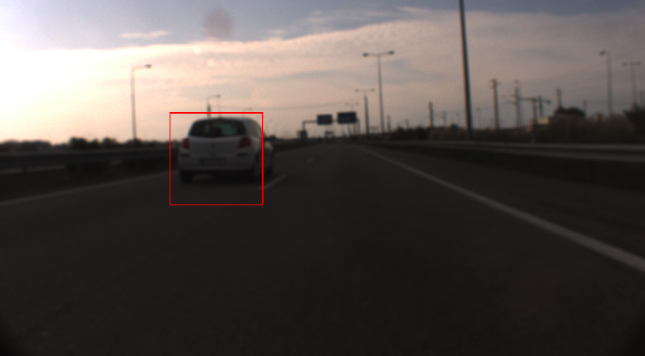
\includegraphics[width=0.49\textwidth]{caplabel/imgs/resultmat.png}\hfill
	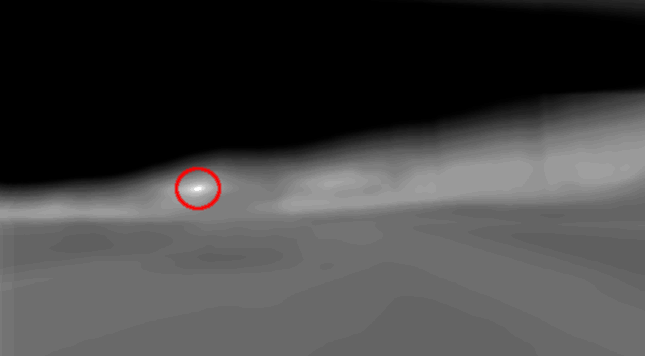
\includegraphics[width=0.49\textwidth]{caplabel/imgs/resultmat2.png}
	
	\caption{Template matching example inverted result matrix}
	\label{fig:resultmat}
	
\end{figure}

For each location, the score is stored in the result matrix. Each location contains a metric score. The brightest points represent the positions where the matching was more similar. In figure \ref{fig:resultmat} two images are displayed: on the left there is an example of a car being selected with a bounding box around it, and on the right is the inverted result matrix from the template matching algorithm. A red circle is around the brightest spot which indicates the location where the matching score was higher. The matching method used for this project is an equation based on the squared difference. The following equation is described by the the following formula

\begin{center}
	$R(x,y) = \sum_{x',y'}(T(x',y')-I(x+x',y+y'))^2$
\end{center}

where $R$ is the result matrix, $T$ is the template (patch, or \gls{roi} in the bounding box) and $I$ is the source image. The result is obtained by calculating the squared difference between the pixels in the template and in the area in that location in the source image.  

After the result matrix is filled, it is needed to locate the highest or lowest value in the result matrix depending on the matching method used. \gls{opencv} implements a function called \texttt{minMaxLoc} which finds the global minimum and maximum in an array or matrix. Because it was used the squared difference as matching method, the locations with highest score are the ones where the difference is minimal.

In other words, the result matrix shows that the place with more similarities is the one where the values are lower. In figure \ref{fig:resultmat} on the right, the result matrix is inverted for demonstration purposes. So in reality, the result matrix for this project show that the location with more similarities is in the position with the lowest value.

It is important to note that after each frame is received, the patch used for the next template matching cycle will be the \gls{roi} acquired in the previous frame. This means that the patch is update when a new frame is received to obtain better accuracy of the object's pose. 

After the whole tracking is done, the back tracking is now performed. The reason why the backward tracking is done after the forward tracking is because if the back tracking would begin when a target is selected in the image before the front tracking, some time would be wasted to process the previous frames, losing some of the next frames used for the front tracking. 

With a queue, the last frames are saved and at the moment of object selection those frames are copied and saved to be processed posteriorly. After the front tracking, the node gets the frames stored before the target selection and applies template matching. With this, the tracking is done in both directions.


\subsection{2D Dataset and Playback}

While tracking objects, the user is prompted to insert a label to the object. The user enters a class to which the object belongs to. The node saves several bounding boxes for each frame. To accomplish this, a bounding box data structure called \texttt{BBox} was implemented.

\begin{figure}
	\begin{center}
		\begin{lstlisting}[label={lst:BBox2d}, caption={BBox struct definition used for 2D datasets.},language=c++]
		struct BBox
		{
			int x;
			int y;
			int width;
			int height;
			int id;
			string label;
		};\end{lstlisting}
	\end{center}
\end{figure}

The \texttt{BBox} struct definition is presented in listing \ref{lst:BBox2d}. The \texttt{BBox} presents its $x$ and $y$ coordinates, its width and height, an id, and a label. While the tracking is performed, several instances of \texttt{BBox} are created and stored in a map that relates the frame with the \texttt{BBox}. 

When the tracking is complete, the user can opt to save the results or to discard them. If the frames are to be saved, the users enters the object label and a folder will be created with patches of the frames where the object appears. The user can also choose to label the objects without saving the templates. In the end, a set of \texttt{BBox} instances are created and a dataset file can be created.

\begin{figure}
	\begin{center}
		\begin{lstlisting}[label={lst:BBox2d_dataset}, caption={2D dataset example snippet},language=c++]
		FRAME_ID 
		BOX_X BOX_Y WIDTH HEIGHT LABEL ID
		...
		1083
		815 663 155 104 car 4
		1084
		816 662 155 104 car 4
		1142
		482 584 152 150 van 5
		1143
		512 589 152 150 van 5
		...\end{lstlisting}
	\end{center}
\end{figure}

The dataset contains, for each frame, a set of bounding boxes that are defined by their coordinates, size, label and object ID. The map where the set of \texttt{BBox} is stored is iterated and printed to a file similar to the snippet in listing \ref{lst:BBox2d_dataset}.

The dataset can be used later to playback the rosbag. Another node was developed with the aim to play the rosbag and identify the objects in the images using the dataset created previously. This rosnode starts similarly to the previous one, by subscribing to the camera \gls{ros} topic and send the image message to a callback function where it is processed. The message is converted into \gls{opencv} format and the dataset file is read. A map similar to the previous is also created to be filled with the dataset information where it relates the objects in the bounding boxes to the frames in the sequence. 

When a frame is received, its frame ID is retrieved. This ID is used to check which boxes in this frame. If this frame contains objects, a rectangle is draw in the image representing the bounding box acquired before. The box also features a legend with the object label and its ID. The color of the bounding box is randomly assigned, depending on its label. In other words, objects with the same label will have the same box color, making it easy to identify objects if the image has several different boxes. The resulting image is presented in figure \ref{fig:playback}. The image is then converted again into the \gls{ros} format and published to a topic.

\begin{figure}[htp]
	
	\centering
	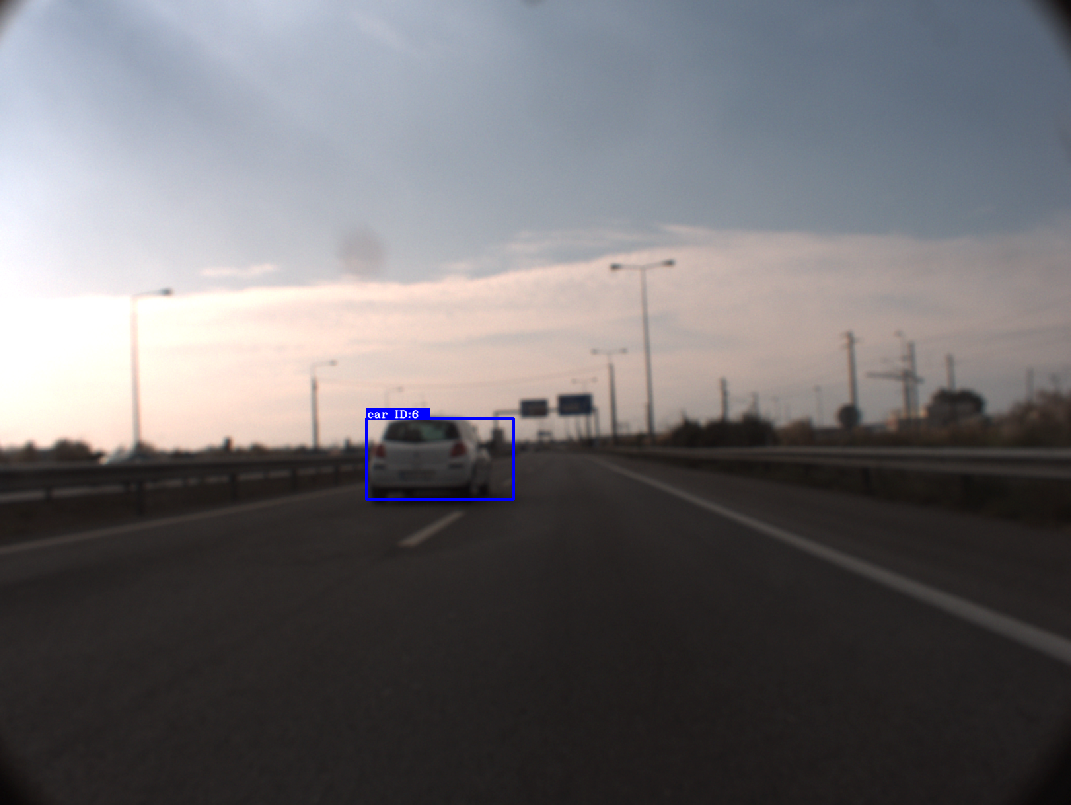
\includegraphics[width=0.8\textwidth]{caplabel/imgs/playback.png}
	
	\caption{Playback example with a car}
	\label{fig:playback}
	
\end{figure}

\section{Range Based Tracking}

After the image processing, the detection, tracking and labelling continues using the \gls{lidar} scanners equipped in the ATLASCAR 2. To develop this part, a continuation to the previous labelling node is added where the capabilities of the laser scans will be explored. The range based object tracking is performed with the \gls{mtt} library developed by Almeida \cite{SoaresDeAlmeida2016a}. 

The \gls{mtt} library was designed specially for the ALTASCAR making it the best tool to be used for this project. The \gls{mtt} works with planar scanners to obtain perception although it receives a pointcloud as input. The \gls{mtt} library supposes that the objects are all at the same height so the pointclouds are flattened. For the scope of this project this is no problem as most of the scanners used are planar except for the SICK LD-MRS. Assuming that the readings of this \gls{lidar} are at the same height does not influence the results as the difference of the measures are minimal. 

\subsection{Multi Target Tracking}

The node starts by subscribing to all topics where \texttt{laserScans} can be found. There are two SICK LMS151, one on each side of the ATLASCAR 2, giving two planar scans with a 270 degree aperture. The SICK LD-MRS features four planar scans. Each scan is submitted into a ROS topic totaling six topics, one for each SICK LMS151 and four topics for the SICK LD-MRS. The six topics are subscribed and the sensor messages are given to a callback function in the \gls{ros} format.

This callback functions gets the laser frame ID. This frame is the transformation frame, not to be misunderstood with an image frame. The frame ID is used to identify the laser scan in the callback function. The callback function converts the \texttt{laserScan} in to a pointcloud.

\begin{figure}[htp]
	
	\centering
	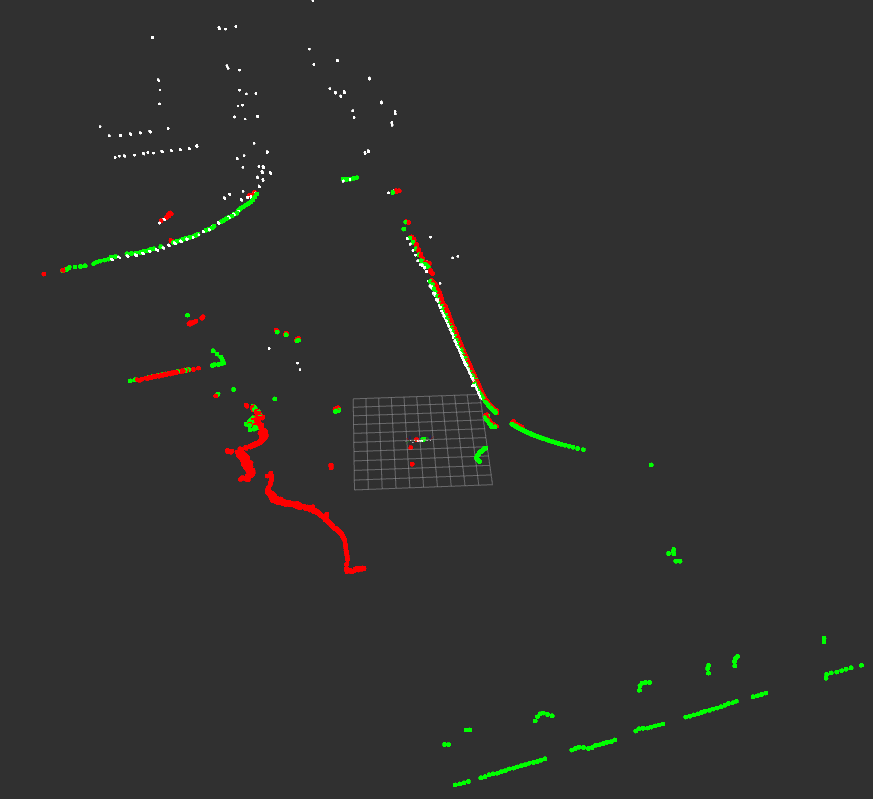
\includegraphics[width=0.6\textwidth]{caplabel/imgs/rviz0.png}
	
	\caption{All the separated laserScans visualized with Rviz}
	\label{fig:rviz0}
	
\end{figure}

In figure \ref{fig:rviz0} the \texttt{laserScans} can be observed individually. The readings from the central SICK LD-MRS are given by the white points. The two SICK LMS151 are distinguished by the red and green colors for the left and right respectively. The colors are chosen regarding nautical and aeronautical navigation lights for port and starboard positions.

In the image callback function, when an image frame arrives it creates a full pointcloud by merging the pointclouds of all \texttt{laserScans}. To do this, a transform listener is created to calculate the transforms at that given time between the two SICK LMS151 and the SICK LD-MRS. The \gls{pcl} library is used here to blend the different \texttt{laserScans}. The \gls{pcl} can concatenate pointclouds with the operator + making it easy to merge them all together. The pointclouds are converted from the \gls{ros} format to \gls{pcl} format, concatenated, and ready to be processed by the \gls{mtt} library. 

Firsty, the final pointcloud is converted to the \gls{mtt} format. The \gls{mtt} library works in a data structure that has all points coordinates called \texttt{t\_data}.

\begin{figure}
	\begin{center}
		\begin{lstlisting}[label={lst:t_data}, caption={t\_data struct definition},language=c++]
		typedef struct
		{
			double x[2160],y[2160];
			double r[2160],t[2160];
			bool flag[2160],flag2[2160];
			bool occlusion_data;
			int initial_position[2160];
			int n_points;
		}t_data; 		\end{lstlisting}
	\end{center}
\end{figure}

The pointcloud is iterated and a \texttt{t\_data} instance is initialized and filled with the pointcloud information. The next step is to cluster the different objects found in the pointcloud. The clustering strategy is implemented by the \gls{mtt} library. The \gls{mtt} takes the full data and initializes a vector of clusters. Clusters are formed by points and its structure contains an id of the cluster, start and end points, total number of points, length of the cluster, among other variables and flags used for occlusion detection.

%\begin{figure}
	\begin{center}
		\begin{lstlisting}[label={lst:stcluster}, caption={st\_cluster struct definition},language=c++]
		struct st_cluster
		{
			///id of the cluster
			int id;			
			///start point
			int stp;
			///end point
			int enp;	
			///total number of points
			int n_points;	
			double rmin,tm;
			double cx,cy,cxp,cyp,cxe,cye;
			double r;
			bool partialy_occluded;
			double lenght;
		};		\end{lstlisting}
	\end{center}
%\end{figure}

The clustering algorithm breaks the data into small groups (clusters) of points. A distance threshold is defined depending on the size of the pointcloud data and the distance between the points is calculated. If the distance between points is greater than the given threshold, then an object is most likely to be there. A set of points near that position will be grouped to form a segment. The clusters are then converted into objects. Objects are defined as a set of lines connecting the points that form the cluster. 

\begin{figure}
\begin{center}
	\begin{lstlisting}[label={lst:stobject}, caption={st\_object struct definition},language=c++]
	struct st_object
	{
		vector<t_linePtr> lines;
		double cx,cy;
		
		double rmin,tm;
		double size;
		
		int id;
		
		bool object_found;
		bool partialy_occluded;
		
		double min_distance_to_existing_object;
	};		\end{lstlisting}
\end{center}
\end{figure}

The lines that form an object are defined by the polar coordinates and the Cartesian coordinates of the initial and final line points.

\begin{figure}
	\begin{center}
		\begin{lstlisting}[label={lst:stline}, caption={st\_line struct definition},language=c++]
		struct st_line
		{
			///Polar coordinates
			double ro,alpha;
			///Initial and final line points
			double xi,yi,xf,yf;
		};		\end{lstlisting}
	\end{center}
\end{figure}


The \gls{mtt} then associates the targets found to a linked list of objects where the full description of the objects are stored. This list is later used to create a motion model where the estimated position of the objects and its velocity is calculated. 

Some objects may become occluded, for example when a car passes in front of another. The \gls{mtt} estimates the position of the occluded objects by creating a motion model using their velocity and so it is possible to track objects while they are out of the field of view but still in the surroundings.

The \gls{mtt} operates around targets. The objects are converted into targets. Targets keep information about the object and its velocity plus their position and obstacle lines. A target list is published to a \gls{ros} topic. 

For the sake of visualization, markers are created and placed in the location fo the objects. For each object in the target list, a marker is created with the ID of the object. The ID increments by one as a new object is found. 

\begin{figure}[htp]
	
	\centering
	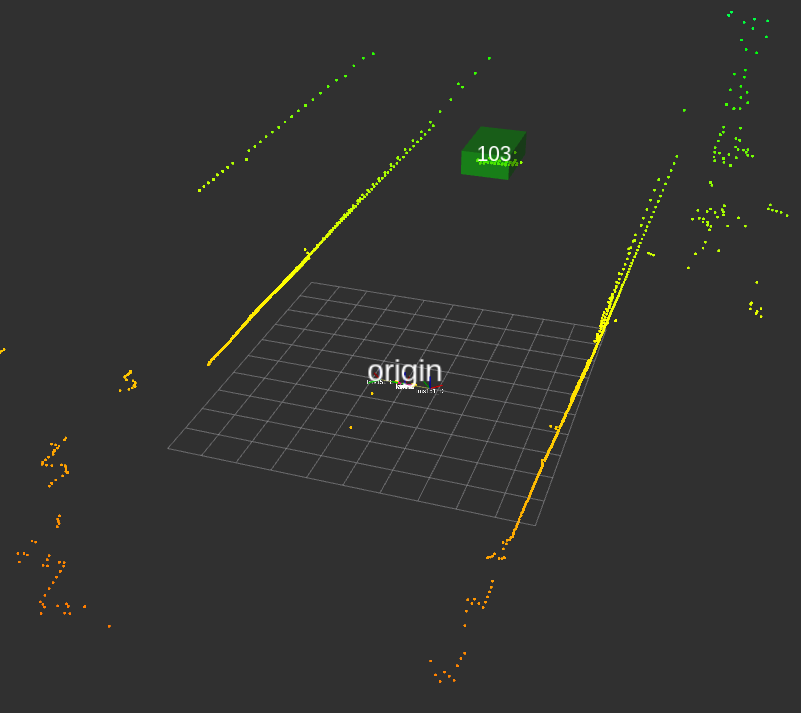
\includegraphics[width=0.65\textwidth]{caplabel/imgs/rviz1.png}
	
	\caption{Visualization of a detected car with \gls{mtt} in Rviz}
	\label{fig:rviz1}
	
\end{figure}

In the position of the object, a visual marker is placed. There are also markers in the form of line strips in order to visualize the connection between the points of the pointcloud. An addition to the marker creation method was made, where 3D bounding boxes are created in the location of the objects.

The information in figure \ref{fig:rviz1} was visualized using the Rviz tool. The \gls{mtt} creates by default a marker at the origin where usually the front of the ATLASCAR 2 is (depending on the transformations). 

In the figure, the processed pointcloud can be seen, where the \gls{lidar} \texttt{laserScans} messages are all merged into. It can also be seen a green 3D bounding box with the ID 103, meaning that an object was found at that location. The object was in fact a car traveling in front of the ATLASCAR 2. 

\subsection{3D Datasets}

To develop datasets and include the 3D information of the tracked targets, some changes have been made to the structure of the \texttt{BBox} in which the 3D coordinates of the objects have been added.

%\begin{figure}
	\begin{center}
		\begin{lstlisting}[label={lst:bbox3d}, caption={BBox struct definition with 3D capabilities},language=c++]
		struct BBox
		{
			int x;
			int y;
			int width;
			int height;
			int id;
			string label;
			// 3D position
			double x3d, y3d, z3d;
		};		\end{lstlisting}
	\end{center}
%\end{figure}

While tracking an object in the image, an object in the \gls{mtt} of ranged based sensors is selected and its ID is retrieved. This object is followed and its position is given to the labelling node to print a dataset file (see listing \ref{lst:dataset3d}) with the full information about the objects whereabouts.

\begin{figure}
\begin{center}
	\begin{lstlisting}[label={lst:dataset3d}, caption={Snippet of the dataset with 3D capabilities},language=c++]
	FRAME_ID
	BOX_X BOX_Y WIDTH HEIGHT LABEL ID 3D_X 3D_Y 3D_Z
	...
	1063
	693 600 218 218 car 1 19.1706 1.64176 0.5
	1064
	692 597 218 218 car 1 19.5359 1.61985 0.5
	1144
	570 597 145 145 van 2 25.7349 2.61821 0.5
	1145
	590 602 145 145 van 2 25.7349 2.61821 0.5
	...		\end{lstlisting}
\end{center}
\end{figure}

The dataset header was updated to contain the 3D information and the contents now present the coordinates in space of the object regarding the ATLASCAR 2 position. Analyzing the snippet in listing \ref{lst:dataset3d}, the \texttt{3D\_Z} values can be seen set to 0.5. The explanation for this is that the \gls{mtt} library implements perception for planar sensors which only give $x$ and $y$ coordinates. For this reason, the height for all objects is estimated as 0.5 (half a meter). 
